\section{Performance issues related to mathematical symbols}
\label{section:symbols}

Since Isabelle is an automated theorem prover, its theory documents require mathematical notation. These notations and other useful symbols are saved in the form of latex-like notations, which are then rendered as Unicode symbols in jEdit and VSCode. For example, the existential quantifier $\exists$ is represented in text form by \texttt{\textbackslash<exists>}. This process makes it easier for people who are used to mathematical notations, such as mathematicians and computer scientists, to read and work on Isabelle documents.

In VSCode, the replacement of the notations is only done visually, which has proven to be quite problematic. This has introduced a number of performance and ergonomic issues for the users, which completely stops them from using Isabelle/VSCode: 
\begin{itemize}
  \item For it to work, a third-party extension needs to be configured, which takes multiple steps in setting up your development environment. 
  \item Every time a new document is opened, the editor becomes completely unresponsive while it is replacing the symbols.
  \item Inserting, deleting, selecting, replacing and navigating through the symbols is inconvenient for the user.
\end{itemize}

Based on anecdotal evidence, these and other issues make working with Isabelle on VSCode unattractive in comparison to its jEdit counterpart.

\paragraph{Current Implementation.}
When the language client is started, a request is sent to the language server asking for the symbol data (name, unicode, tag). This data is then processed by the client and a third-party extension, Prettify Symbols Mode, is started. The symbol  replacements are then registered which allow the third-party extension to start replacing. Each Isabelle or Isabelle/ML file that is opened will have its latex notations replaced with the respective Unicode symbol. This process is illustrated below in \autoref{fig:sequence-psm}.

\begin{figure}[htb]
  \centering
  \begin{sequencediagram}
    \newthread{A}{Language Client}{}
    \newinst[1.5]{B}{Language Server}{}
    \newinst[1.5]{C}{Prettify Symbols Mode}{}
    
    \begin{call}{A}{Request Symbols}{B}{Symbol Data}
        \postlevel
    \end{call}
    
    \postlevel

    \begin{call}{A}{Process Symbols}{A}{}
        \postlevel
    \end{call}

    \begin{call}{A}{Activate}{C}{}
    \end{call}
    
    \postlevel
    
    \begin{messcall}{A}{Register Replacements}{C}{}
        \postlevel
    \end{messcall}

    \begin{sdblock}{Open File}{}
        \begin{messcall}{C}{Decorate Symbols}{C}{}
            \postlevel
        \end{messcall}
    \end{sdblock}
  \end{sequencediagram}

  \caption{Sequence diagram representing the steps for symbol rendering with Prettify Symbols Mode.}
  \label{fig:sequence-psm}
\end{figure}

Internally, Prettify Symbols Mode finds all the ranges in the text document with the latex notations. It manages to hide the text inside these ranges by applying CSS decorations such as making the font size really small or setting letter spacing to a negative value. Then using the CSS pseudo-element \texttt{after}, it shows the corresponding Unicode symbol after the hidden text.

\paragraph{Solutions.}
The VS Code Extension API provides a number of different endpoints to tackle this problem, but most of them are not suitable to solve it without using them in unintended ways. The following VSCode interfaces were considered:
\begin{itemize}
  \item \textbf{Decorations.} The decorations API is used to apply CSS to different text sections. This is the API that Prettify Symbols Mode uses to solve the symbols problem. The creator of this extension, \citeauthor{psm_issue}, was also trying to solve the same problem but with a different theorem prover, namely the COQ Proof Assistant. He stopped updating the extension around 2017, and since then the decorations API was not updated in any meaningful way~\parencite{psm_issue}. That's why trying to use this API would be futile, since in the end it would not solve our problems, similar to Prettify Symbols Mode. 
  \item \textbf{Virtual Document.} This API allows one to create virtual documents from sources which can then be displayed in the editor. But, these documents are unfortunately read only.
  \item \textbf{Custom Editor.} The custom editor could have been a suitable solution since it allows the user to manipulate the byte stream and display it to the user how you see fit. The problem with it is that we would have to implement the whole editor in HTML, which would require a lot of effort and would break the functionality of other extensions.
  \item \textbf{Custom Notebook.} Notebooks are more powerful versions of the custom editors. However, custom notebooks are still under development so it would be to risky to use them and they would most probably not fix the issue. 
  \item \textbf{File System Provider.} This API is meant to enable extensions to serve files from remote places, like ftp-servers, and to seamlessly integrate those into the editor. It allows extensions to provide a file system for schemes other than "file:". Since with it we can define all the useful operations, such as \texttt{read}, \texttt{write}, etc, it was the most suitable candidate for us. The only downside is that we would have to generate an Isabelle view on the theory files and store them in memory, parallel to the original disc files.
\end{itemize}

Other potential approaches:
\begin{itemize}
  \item \textbf{Character Encoding.} Isabelle/jEdit uses encoding to solve the symbols problem. It provides its own charset UTF-8-Isabelle, where all the latex notations are encoded to the correct symbols. In VSCode, although you can set the encoding of the document, you cannot provide your own charset. 
  \item \textbf{Font Ligatures.} Normally, a ligature occurs when two or more letters are joined as a single glyph. An example would be when the characters a and e are joined together to form the glyph \ae. We briefly considered building our own font with custom ligatures mapped to our latex notations. This approach has the same pitfalls as Prettify Symbols Mode, for example the \texttt{search and replace} function would also affect the text inside our ligatures. 
\end{itemize}

\subsubsection*{The Isabelle File System}
To implement our file system, we introduced the "isabelle:" scheme. The implementation of the file system consists mainly of 3 modules: \emph{IsabelleFSP}, \emph{SymbolEncoder} and \emph{PrefixTree}. The relation between these modules is illustrated in \autoref{fig:class_diagram}.

\texttt{IsabelleFSP} (FSP short for \emph{FileSystemProvider}) implements the VSCode \texttt{FileSystemProvider} interface. \texttt{IsabelleFSP} uses the Singleton design pattern and only makes public static functions such as \texttt{register}, to register its single instance as a file system, \texttt{initWorkspace}, to setup the workspace, and other less relevant functions. \\
\texttt{SymbolEncoder} encodes the byte streams according to the mapping of latex notations to symbols.\\
\texttt{PrefixTree} stores the search tree for byte sequences and their replacement values, for fast symbol recoding.\\

\begin{figure}[ht]
\centering
\begin{tikzpicture}
\begin{umlpackage}{Isabelle File System}
\umlinterface[]{vscode::FileSystemProvider}{}{
    read(Uint8Array): Uint8Array \\
    write(Uint8Array) \\
    ...
}
\umlclass[y=-4]{IsabelleFSP}{
    instance: IsabelleFSP \\
    symbolEncoder: SymbolEncoder
}{
    register(context: ExtensionContext)
}
\umlunicompo[mult=1, pos=0.7, angle1=-30, angle2=-60, loopsize=2cm]{IsabelleFSP}{IsabelleFSP}

\umlimpl[]{IsabelleFSP}{vscode::FileSystemProvider}

\umlclass[y=-8.5]{SymbolEncoder}{
    sequences: EncodeData \\
    symbols: EncodeData
}{
    encode(data): Uint8Array \\
    decode(data): Uint8Array
}
\umlaggreg[mult=1, pos=0.8, angle1=30, angle2=60, loopsize=2cm]{IsabelleFSP}{SymbolEncoder}

\umlclass[x=8,y=-8.5]{EncodeData}{
  prefixTree: PrefixTree \\
  minLength: number \\
  maxLength: number 
}{}
  
\umlaggreg[mult=2]{SymbolEncoder}{EncodeData}


\umlclass[x=8, y = -4]{PrefixTree}{
    root: TreeNode
}{
    getNode(prefix)
}
\umlunicompo[mult=1]{EncodeData}{PrefixTree}

\umlclass[x=8]{TreeNode}{
    key: number \\
    value: number[] \\
    end: boolean \\
    children: <number, TreeNode>
}{}
\umlunicompo[mult=1]{PrefixTree}{TreeNode}

\end{umlpackage}
\end{tikzpicture}
\caption{Class diagram of Isabelle file system (only important class properties shown for brevity)}
\label{fig:class_diagram}
\end{figure}

When the extension is activated, the \texttt{IsabelleFSP} registers its instance to VSCode and it also creates a new workspace folder for the Isabelle memory files. This is done before the server is activated, because if the first workspace folder is added, removed or changed, the currently executing extensions (including the one that called this method) will be terminated and restarted. If we do this after we get a response from the server, it would cause the server to restart which would lead to an even greater startup time.

\texttt{IsabelleFSP}, aside from that, also registers a function that is executed when a document has been opened. This function checks if the document is an Isabelle theory file and then creates a mirroring memory file on the Isabelle scheme. In \texttt{IsabelleFSP} a mapping of URIs is saved between the disc files and the memory files. The byte array of the old file is read and then it is encoded by the \texttt{SymbolEncoder}. When changes are written to the memory file, then they will be synced with its original file after they are decoded and vice versa.

There is only one instance of the \texttt{SymbolEncoder} which is created after we get a response from the server with the symbol data. Using the data the \texttt{SymbolEncoder} creates two \texttt{EncodeData} objects, namely \texttt{symbols} and \texttt{sequences}. These objects contain a Prefix Tree, the smallest and largest length of the words. Because in JavaScript, the byte arrays from files are represented in number arrays, it was practical to make a \texttt{PrefixTree} which works with the type of number array. Each node on the tree has a number as the \texttt{key}, a \texttt{children} map, and a \texttt{boolean end}, which tells us if it is the last node. If it is an end node, it also has the value of the number array it is supposed to be replaced with. This process is described below in \autoref{algo:symbol-encoder}. Inside the \texttt{SymbolEncoder}, encoding and decoding work exactly the same way as they just call the \texttt{coding} function only with a different \texttt{EncodingData} object. 
%When we encode we use the object sequences because we are encoding character sequences to unicode symbols. For decoding, we use the object symbols.

\begin{algorithm}[H]
\SetAlgoLined
\caption{Algorithm used for encoding and decoding of byte arrays.}
\label{algo:symbol-encoder}
\KwIn{Number array A of length $l$, Object B of type EncodeData}
\KwResult{Number array C}
\For{$i \leftarrow 0$ \KwTo $l$}{
    $word \leftarrow [ ]$\;
    $node: TreeNode$\;
    \For{$j \leftarrow i$ \KwTo $i + B.maxLength$}{
        word.push(A[j])\;
        $node \leftarrow B.prefixTree.getNode(word)$\;
        \If{No node found or node is an end node}{
            break\;
        }
    }
    \eIf{node is defined and is end node}{
        $C \leftarrow C.concat(node.value)$\;
        $i \leftarrow i + word.length$\;
    }{
        C.push(A[i])\;
    }
}
\end{algorithm}

A special case of rendering which could not be handled by Unicode was superscript and subscript text. Unicode does not have all characters in these modes. For this reason, this had to be done through CSS decorations, similarly to Prettify Symbols Mode. Since these are only 2 decoration types, one to show the text as superscirpt and one as subscript, it doesn't affect performance the way Prettify Symbols Mode did.

Now, we have to develop a mechanism for adding files to the Isabelle file system. The first alternative is, as soon as one opens a *.thy file that file is then closed, its encoded version is added to the Isabelle file system, and then its opened/shown to the user. Although this solution is simple in theory, implementing it presents a number of problems:
\begin{itemize}
    \item The new file has its own URI, with the scheme "isabelle:", which is not accepted by the backend. For the backend to correctly function, it requires the disc file URIs, which use the scheme "file:". 
    \item The new file has no decorations, as a result of being marked as a draft.
    \item Organizing the files added to our file system in directories, that mirror the directories of the disc file system, clutters our workspace. The user would then have to navigate through multiple directories and subdirectories to find a theory file.
\end{itemize}

Because the user is now expected to work exclusively with the files on the Isabelle file system, we can completely remove communication between client and server when a normal theory file is opened/modified/etc. Instead, all requests and notifications from "isabelle:" files are now caught by a middleware and then their URI is translated to the URI of the disc file that they represent, before being sent to the server and vice-versa. This procedure works as described below in \autoref{fig:uritranslate}. This way the server can process the Isabelle file system files and the client gets back the decorations, highlighting, and all the other features.

We still have the problem of when and which files to add to the Isabelle file system. To do this we can use the formal document model, where theory files belong to a certain Isabelle session. We can mirror the formal model on the Isabelle file system, which would be advantageous for users who are already used to this directory structure. This is also somewhat similar to the theories panel in Isabelle/jEdit.

When the extension is activated, we send to the server the current directory. Usually Isabelle projects have a ROOT or ROOTS file which is a configuration file, to mark the needed theory files for one or multiple sessions. The server then checks the directory for the ROOT file and makes a list of all the session and their theory files. This list is sent to the client which then adds all these files to the Isabelle file system in a directory with the name of the responsible session. When the user opens files that do not belong to any of the the sessions in the ROOT files, these files get added to the Draft session. 

\begin{figure}[htbp]
  \centering
  \begin{sequencediagram}
    \newthread{A}{Language Client}{}
    \newinst[1.5]{B}{Middleware}{}
    \newinst[1.5]{C}{Language Server}{}
    
    \begin{call}{A}{Activate with current directory}{C}{}
    \end{call}
    \postlevel
    \begin{call}{A}{Request Symbols}{C}{}
    \end{call}
    \postlevel
    \begin{call}{A}{Request Theories}{C}{}
    \end{call}
    
    \postlevel

    \begin{call}{A}{Create Encoded Files}{A}{}
    \end{call}
    
    \begin{sdblock}{All other requests}{}
        \begin{call}{A}{Request}{B}{}
            \begin{call}{B}{Translate URI}{B}{}
            \end{call}
                
            \begin{call}{B}{Request}{C}{}
            \end{call}
            
            \begin{call}{B}{Retranslate URI}{B}{}
            \end{call}
        \end{call}
    \end{sdblock}
  \end{sequencediagram}

  \caption{Sequence diagram describing the URI translation with the middleware.}
  \label{fig:uritranslate}
\end{figure}

At this stage, when the user reopens a previously initialized Isabelle workspace, the workspace needs to wait for the server to start so that it can be repopulated with the appropriate files. This can take a while and the user cannot work on anything during this time. Also the user will lose the arrangement of the previously opened documents, which can be frustrating for the user to work with. To circumvent this, we need to save the state of our workspace and initialize it with this saved state while we wait for the server to start. Instead of saving the contents of the theory files, which can be pretty large, we only need to save the current configuration of our \texttt{SymbolsEncoder} and the paths of the files that we need.

\subsection*{Results}
The Isabelle experience in VSCode is much closer to jEdit. Symbols can now be added, deleted, edited the same as any other characters. As opposed to Prettify Symbols Mode, where the editor would react unpredictably when manipulating symbols. 

The editor freezing problem, which was also caused by Prettify Symbols Mode, is solved. For large files like \emph{HOL/List.thy} or when trying to open imports, the extension would hang noticeably. This didn't happen only on the first time a document is opened but even when changing from one open document to another open document. Now the files are encoded once, when they are added to the Isabelle file system, and after that there are no more computations to be made. So opening or switching between windows is instantaneous. 

A slight disadvantage that our solution might have is that it may use more RAM to store all the encoded theory files. Also, some users might be confused by having two workspace folders. The workspace arrangement can be seen in \autoref{fig:workspace-old} and \autoref{fig:workspace-new}.  To mitigate the second problem we have dialog boxes informing the user in which file system he is operating.

To keep the models consistent we had to implement a two way synchronisation between the theory files and the disc files. This means that changes to the one are reflected on the other and vice-versa. While this works perfectly fine most of the time, it breaks down when the disc file is not in the workspace. In that case only changes from the theory file will be reflected on the disc file, but not the other way around. This is due to the limitations that VSCode sets on the extensions, allowing them to only catch events for files inside the workspace.

% \begin{figure}[htbp]
%   \centering
%   \subfloat[Old][Old editor]{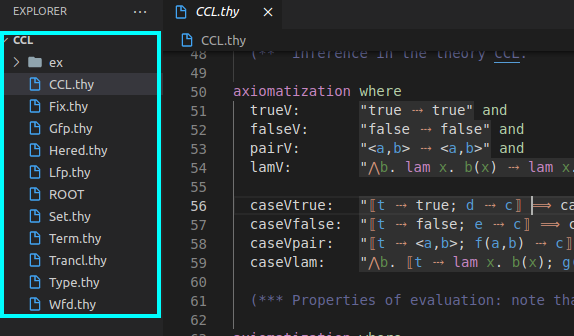
\includegraphics[width=0.45\textwidth]{figures/problem2/old_editor_rectangle.png}}
%   \hfill
%   \subfloat[New][New editor]{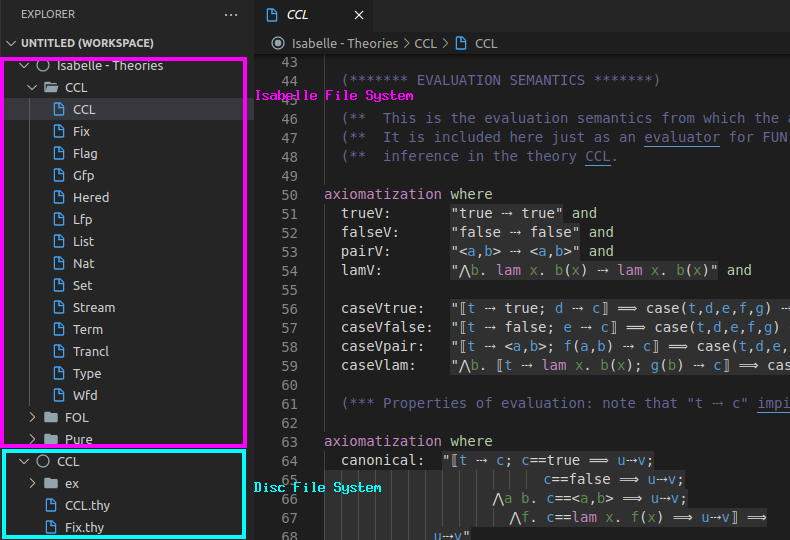
\includegraphics[width=0.45\textwidth]{figures/problem2/new_editor_annotated.png}}
%   \caption{Two TUM pictures side by side.}
% \end{figure}

\begin{figure}[htbp]
    \centering
    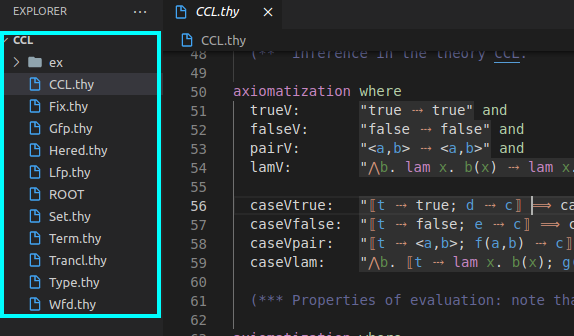
\includegraphics[width=0.8\textwidth]{figures/problem2/old_editor_rectangle.png}
    \caption{VSCode editor with one workspace folder for the "file:" file system.}
    \label{fig:workspace-old}
\end{figure}
\begin{figure}[htbp]
    \centering
    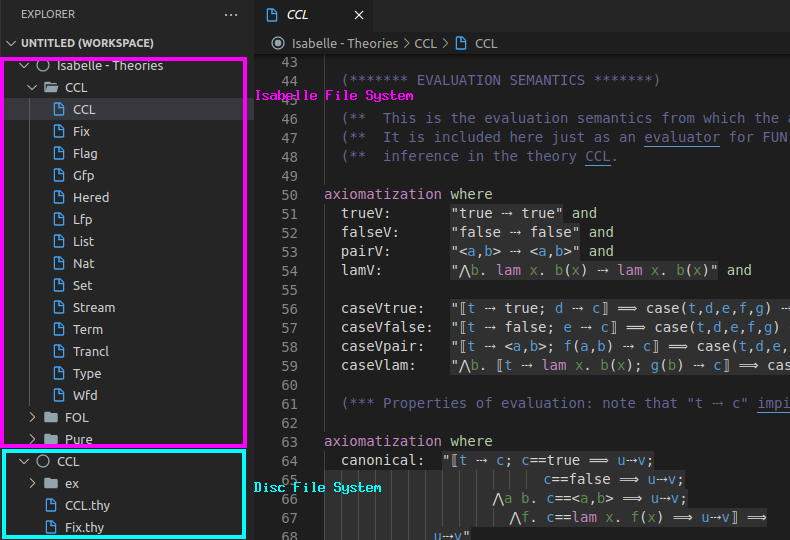
\includegraphics[width=0.8\textwidth]{figures/problem2/new_editor_annotated.png}
    \caption{VSCode editor with two workspace folder for different file systems ("isabelle:" and "file:").}
    \label{fig:workspace-new}
\end{figure}